\documentclass[conference]{IEEEtran}
\IEEEoverridecommandlockouts

\usepackage{cite}
\usepackage{amsmath,amssymb,amsfonts}
\usepackage{graphicx}
\usepackage{textcomp}
\usepackage{xcolor}
\usepackage{booktabs}
\usepackage{url}

\begin{document}

\title{Quantization and Pruning of Small Language Models: Decoupling Contextual Representation Collapse from Downstream Task Robustness}

\author{
    \IEEEauthorblockN{Shikhar Veeramachineni}
    \IEEEauthorblockA{\textit{School of Computer Science and Engineering} \\
    \textit{VIT-AP University} \\
    Amaravati, India \\
    Reg. No: 23BCE9278 \\
    shikhar.23bce9278@vitapstudent.ac.in}
    \and
    \IEEEauthorblockN{Jessea Thomas Jaison}
    \IEEEauthorblockA{\textit{School of Computer Science and Engineering} \\
    \textit{VIT-AP University} \\
    Amaravati, India \\
    Reg. No: 23BCE9291 \\
    jessea.23bce9291@vitapstudent.ac.in}
}

\maketitle

\begin{abstract}
Model compression via weight pruning and post-training quantization is vital for deploying transformer-based Language Models (LMs) to resource-constrained edge devices. However, prior literature frequently conflates downstream task accuracy on fine-tuned classification heads with the preservation of foundational latent language modeling representations. In this study, we conduct an extensive, reproducible empirical investigation on DistilBERT ($66.98\text{M}$ parameters), cleanly decoupling two distinct evaluation tracks: (1)~\textbf{Track A:} Base contextual representation and semantic geometry preservation using 16 multi-domain masked language modeling (MLM) probes and 5 semantic sentence pairs across four pruning paradigms (Local $L_1$, Global $L_1$, Structured $L_n$ channel, and Random) and multi-bit precisions (FP32, Dynamic INT8, Simulated INT4); and (2)~\textbf{Track B:} Task-specific sequence classification robustness and single-socket CPU inference latency profiling on SST-2 ($N=60$ validation sentences) across eight pruning levels ($0\%$ to $50\%$). Our findings establish that: (i)~Contextual representation exhibits an abrupt non-linear collapse cliff at $\approx 45\%\text{--}50\%$ sparsity, where Global $L_1$ retains $87.50\%$ Top-1 token prediction accuracy while Structured $L_n$ plummets to $31.25\%$; (ii)~Global pruning inherently protects attention Key/Query projections ($38.2\%\text{--}42.8\%$ sparsity) while allocating over $51.4\%\text{--}55.4\%$ sparsity to feed-forward networks (FFNs); (iii)~On standard CPU architectures, unstructured pruning yields \textit{zero wall-clock latency speedup} ($0.91\times\text{--}1.01\times$) due to dense BLAS execution overheads, whereas Dynamic INT8 quantization delivers a deterministic $1.67\times\text{--}1.70\times$ speedup ($91.51\text{ ms} \to 54.90\text{ ms}$) and a $48.20\%$ disk footprint reduction ($255.45\text{ MB} \to 132.29\text{ MB}$); and (iv)~Post-pruning knowledge distillation effectively recovers accuracy at the collapse cliff ($81.25\% \to 93.75\%$, $+12.50\text{ pp}$). We provide definitive architectural trade-offs and deployment guidelines for edge NLP pipelines.
\end{abstract}

\begin{IEEEkeywords}
Model Compression, Neural Network Pruning, Post-Training Quantization, Small Language Models, DistilBERT, Latent Space Geometry, CPU Edge Inference.
\end{IEEEkeywords}

\section{Introduction}
Pre-trained bidirectional transformer architectures, such as BERT~\cite{devlin2018bert} and DistilBERT~\cite{sanh2019distilbert}, have become the de facto foundation for contemporary Natural Language Processing (NLP). However, their substantial computational complexity, memory bandwidth demands, and parameter footprints impede real-time execution on resource-constrained platforms, including mobile edge hardware, IoT microprocessors, and automotive embedded systems. Consequently, neural model compression techniques---predominantly network pruning~\cite{han2015learning,han2016deep,frankle2018lottery} and post-training quantization~\cite{jacob2018quantization,nagel2021white,dettmers2022llm}---have become indispensable.

Despite prolific research in neural network compression, three critical empirical disconnects persist in current literature:
\begin{enumerate}
    \item \textbf{Metric Disconnect (Task Accuracy vs. Contextual Geometry):} Most existing studies evaluate model compression exclusively on downstream task accuracy (e.g., GLUE benchmarks~\cite{wang2018glue}). Task-specific heads can mask severe internal latent representation decay, creating an illusion of robustness while underlying contextualization, masked-token prediction, and syntactic fidelity degrade catastrophically~\cite{hooker2019compressed}.
    \item \textbf{Hardware-Sparsity Disconnect:} While theoretical FLOP reductions scale linearly with unstructured weight pruning, standard commodity edge hardware lacks specialized sparse matrix multiplication (SpMM) execution units. Consequently, sparse models executed via dense BLAS libraries incur full arithmetic operations or suffer memory overheads, yielding zero runtime acceleration~\cite{hooker2020hardware}.
    \item \textbf{Quantization-Pruning Compounding Effects:} Pruning alters weight distribution variances, creating extreme outliers that can compromise subsequent uniform integer quantization grids, leading to unpredictable compounding degradation across multi-bit precision spectrums (FP32 $\to$ FP16 $\to$ INT8 $\to$ INT4).
\end{enumerate}

To rigorously address these issues, this paper presents a controlled, verifiable empirical evaluation across two cleanly decoupled experimental tracks:
\begin{itemize}
    \item \textbf{Track A (Pre-trained Masked-Token Contextual Preservation):} Using the base pre-trained \texttt{distilbert-}\allowbreak\texttt{base-}\allowbreak\texttt{uncased} model ($66.98\text{M}$ parameters), we evaluate the degradation of contextual language modeling, semantic sentence embedding drift, and layer-wise sensitivity across four pruning paradigms (Local $L_1$, Global $L_1$, Structured $L_n$, and Random) and three quantization precisions (FP32, Dynamic INT8, Simulated INT4).
    \item \textbf{Track B (Fine-Tuned Sequence Classification \& CPU Benchmark):} Using \texttt{distilbert-}\allowbreak\texttt{base-}\allowbreak\texttt{uncased-}\allowbreak\texttt{finetuned-}\allowbreak\texttt{sst-2-}\allowbreak\texttt{english} ($66.96\text{M}$ parameters), we conduct a rigorous 50-iteration CPU latency benchmark and evaluate classification robustness across eight sparsity levels ($0\%$ to $50\%$) under FP32 and Dynamic INT8.
\end{itemize}

Specifically, this study answers five central Research Questions (RQs):
\begin{itemize}
    \item \textbf{RQ1 (Representation Collapse Cliff):} At what exact sparsity threshold does contextual representation collapse occur across different pruning regimes?
    \item \textbf{RQ2 (Architectural Sensitivity and Submodule Allocation):} How does non-uniform global pruning allocate sparsity between Multi-Head Self-Attention (MHSA) and Feed-Forward Networks (FFN)?
    \item \textbf{RQ3 (Multi-Bit Precision Spectrum Boundary):} What are the storage, accuracy, and fidelity limits when transitioning from FP32 to Dynamic INT8 and Simulated INT4?
    \item \textbf{RQ4 (Distillation Recovery Efficacy):} Can post-pruning distillation using a dense teacher recover representation loss at the collapse boundary?
    \item \textbf{RQ5 (The Hardware-Sparsity Disconnect):} How does measured CPU wall-clock latency correlate with theoretical sparsity, and does integer quantization resolve the memory bandwidth bottleneck?
\end{itemize}

\section{Related Work}
\subsection{Transformer Sparsification and Pruning}
Neural network pruning eliminates redundant parameters while preserving task performance. Han et al.~\cite{han2015learning} pioneered magnitude-based pruning for convolutional networks. Gordon et al.~\cite{gordon2020compressing} extended unstructured magnitude pruning to BERT, demonstrating that pre-trained representations exhibit high compressibility during transfer learning. Frankle and Carbin's Lottery Ticket Hypothesis~\cite{frankle2018lottery} and its subsequent transformer extensions~\cite{chen2020lottery} revealed sparse sub-networks capable of matching full-model accuracy. Structured pruning approaches~\cite{michel2019sixteen,voita2019analyzing} remove entire attention heads or FFN channels, aiming to provide hardware-friendly regular structures at the expense of higher accuracy loss.

\subsection{Quantization of Deep Neural Networks}
Quantization reduces numerical precision of weights and activations from 32-bit floating point (FP32) to lower-bit representations~\cite{jacob2018quantization,nagel2021white}. Dynamic post-training quantization (PTQ) statically quantizes weights to 8-bit integers while dynamically quantizing activations at runtime, effectively halving memory bandwidth bottlenecks with minimal degradation on CPU architectures~\cite{zafrir2019q8bert,bhandare2019efficient}. Recent work in generative language models focuses on 4-bit weight-only schemes~\cite{frantar2022gptq,lin2023awq}. However, the compounding interaction of aggressive unstructured pruning followed by dynamic quantization on contextual transformer representations remains under-explored.

\subsection{Knowledge Distillation and Task Decoupling}
Knowledge distillation~\cite{hinton2015distilling} transfers predictive dark knowledge from an overparameterized teacher network to a compact student network. DistilBERT~\cite{sanh2019distilbert} compressed BERT by $40\%$ while retaining $97\%$ of its language understanding using triple-loss distillation during pre-training. Subsequent architectures, such as TinyBERT~\cite{jiao2019tinybert} and MiniLM~\cite{wang2020minilm}, incorporated intermediate hidden-state and self-attention relation alignment. In this work, we deploy lightweight post-pruning distillation to specifically evaluate whether representation damage sustained at the sparsity collapse cliff can be reversed without full re-training.

\begin{table*}[!t]
\caption{Systematic Comparison Between Experimental Implementations (Track A vs. Track B)}
\label{tab:implementation_comparison}
\centering
\resizebox{\textwidth}{!}{%
\begin{tabular}{p{4.2cm}p{6.5cm}p{6.5cm}}
\hline
\textbf{Architectural \& Experimental Dimension} & \textbf{Track A: Masked-Token Context Representation} & \textbf{Track B: Fine-Tuned SST-2 Sequence Classification} \\
\hline
HuggingFace Checkpoint & \texttt{distilbert-base-uncased} & \texttt{distilbert-base-uncased-}\allowbreak\texttt{finetuned-sst-2-english} \\
Target Task & Masked Language Modeling (MLM) & Binary Sentiment Classification \\
Output Head Architecture & Transform + LayerNorm + Vocab Proj (30,522 classes) & Pre-Classifier (768) + Dropout + Classifier (2 classes) \\
Head Parameters & 23,885,306 parameters (622,650 unique tied) & 592,130 parameters \\
Total Model Parameters & 66,985,530 parameters & 66,955,010 parameters \\
Evaluation Dataset & 16 Multi-Domain Probes \& 5 Semantic Pairs & SST-2 Validation Subset ($N=60$ examples) \\
Evaluation Metrics & Top-1 / Top-5 Token Acc., Mean Cosine Similarity & Classification Accuracy (\%), Prediction Drift \\
Pruning Regimes & Local $L_1$, Global $L_1$, Structured $L_n$, Random & PyTorch Unstructured $L_1$ on Linear modules \\
Evaluated Sparsity Grid & 0\%, 15\%, 30\%, 45\%, 60\%, 75\% & 0\%, 10\%, 20\%, 25\%, 30\%, 35\%, 40\%, 50\% \\
Quantization Schemes & FP32, Dynamic INT8, Simulated INT4 & FP32, Dynamic INT8 (\texttt{torch.ao.quantization}) \\
Inference Input Format & Dynamic sequence lengths (12 to 28 tokens) & Fixed tokenized tensor: $[1, 64]$ \\
Latency Benchmark Protocol & $N=50$ iterations, $W=5$ warmup, CPU & $N=50$ iterations, $W=5$ warmup, \texttt{perf\_counter}, CPU \\
Distillation Recovery & Implemented (Teacher-Student Masked KD, 45\%) & Not evaluated in base classification suite \\
Serialized Disk Size & FP32: 255.57 MB, INT8: 154.76 MB ($-$39.5\%) & FP32: 255.45 MB, INT8: 132.29 MB ($-$48.2\%) \\
Primary Objective & RQ1--RQ5: Semantic Geometry \& Submodule Collapse & Classification Robustness \& Real-World CPU Latency \\
\hline
\end{tabular}%
}
\end{table*}


\section{Model Architectures and Experimental Setup}
\subsection{Architectural Demarcation: Track A vs. Track B}
To prevent methodological conflation, we formally distinguish the two models and experimental tracks evaluated in this study, summarized in Table~\ref{tab:implementation_comparison}.

\textbf{Track A} evaluates the pre-trained masked language model checkpoint \texttt{distilbert-base-uncased} on multi-domain contextual probes and semantic embedding similarity. The model comprises a 6-layer transformer encoder followed by a pre-training MLM head consisting of a dense projection ($768 \times 768$), GeLU activation, LayerNorm, and a tied vocabulary projection matrix ($30,522 \times 768$).

\textbf{Track B} evaluates the task-specific sequence classification checkpoint \texttt{distilbert-}\allowbreak\texttt{base-}\allowbreak\texttt{uncased-}\allowbreak\texttt{finetuned-}\allowbreak\texttt{sst-2-}\allowbreak\texttt{english} on 60 validation sentences from the Stanford Sentiment Treebank (SST-2)~\cite{socher2013recursive}. Here, the MLM head is replaced by a sequence classification pooling head: a pre-classifier linear layer ($768 \times 768$), ReLU activation, dropout ($p=0.2$), and a 2-class linear classifier ($2 \times 768$).

\subsection{Parameter Accounting and Submodule Taxonomy}
Accurate parameter accounting is mandatory for reproducible sparsification. Table~\ref{tab:parameter_accounting} presents the exact parameter distribution of the DistilBERT transformer encoder.

\begin{table}[!t]
\caption{DistilBERT Architectural Parameter Accounting and Submodule Taxonomy}
\label{tab:parameter_accounting}
\centering
\resizebox{\columnwidth}{!}{%
\begin{tabular}{lcccc}
\hline
\textbf{Submodule Component} & \textbf{Modules} & \textbf{Weight Shape} & \textbf{Parameters} & \textbf{Fraction (\%)} \\
\hline
Word \& Position Embeddings & 3 & $[30522, 768], [512, 768]$ & 23,835,648 & 35.58\% \\
Attention Projections ($Q, K, V$) & 18 & $6 \times [768, 768] \times 3$ & 10,616,832 & 15.85\% \\
Attention Output Dense & 6 & $6 \times [768, 768]$ & 3,538,944 & 5.28\% \\
FFN Intermediate Layer 1 & 6 & $6 \times [3072, 768]$ & 14,155,776 & 21.13\% \\
FFN Output Layer 2 & 6 & $6 \times [768, 3072]$ & 14,155,776 & 21.13\% \\
Layer Normalizations & 13 & $13 \times [768] \times 2$ & 19,968 & 0.03\% \\
MLM Transformation Layer & 1 & $[768, 768]$ & 589,824 & 0.88\% \\
MLM Vocab Projector (Tied) & 1 & $[30522, 768]$ & (Tied to Embed) & --- \\
\hline
\textbf{Total Transformer Encoder} & \textbf{36} & --- & \textbf{42,467,328} & \textbf{63.40\%} \\
\textbf{Total DistilBERT Architecture} & --- & --- & \textbf{66,985,530} & \textbf{100.00\%} \\
\hline
\end{tabular}%
}
\end{table}


Across the 6 encoder layers, the model possesses exactly 36 Linear modules ($42,467,328$ parameters), divided into:
\begin{itemize}
    \item \textbf{Attention Projections (MHSA):} 18 linear layers ($Q, K, V$) totaling $10,616,832$ parameters ($15.85\%$).
    \item \textbf{Attention Output Dense:} 6 linear layers totaling $3,538,944$ parameters ($5.28\%$).
    \item \textbf{Feed-Forward Network (FFN):} 12 linear layers (\texttt{lin1} and \texttt{lin2}) totaling $28,311,552$ parameters ($42.27\%$).
\end{itemize}
In Track A, the inclusion of the MLM head brings the total linear parameter count to $66,498,048$ across 38 modules ($66,985,530$ total parameters). In Track B, the compact 2-class classification head contains only $592,130$ parameters, yielding $66,955,010$ total parameters. This architectural divergence directly explains why the serialized Dynamic INT8 checkpoint size is $154.76\text{ MB}$ in Track A but $132.29\text{ MB}$ in Track B: the classification checkpoint avoids storing a dynamically quantized $30,522$-class projection matrix.

\subsection{Environment Setup and Deterministic Reproducibility (Step 1)}
To guarantee strict scientific reproducibility across heterogeneous execution environments, all software dependencies were systematically pinned: \texttt{transformers} ($\ge 4.40.0$), \texttt{torch} ($2.6.0$), \texttt{datasets}, \texttt{accelerate}, \texttt{gradio}, \texttt{scikit-learn}, and \texttt{seaborn}. A universal pseudo-random seed ($42$) was globally established across PyTorch, NumPy, and Python runtime environments. Single-thread CPU thread allocation (\texttt{torch.set\_num\_threads(1)}) was enforced during latency profiling to eliminate multi-threaded scheduling jitter, with hardware environments cross-validated on an NVIDIA T4 GPU platform and an x86-64 host processor.

\subsection{Linguistic Evaluation Suite and Semantic Geometry (Step 3)}
To evaluate latent representations independently of task-specific classification heads, we curated a multi-domain contextual probing suite comprising 16 masked-token sentences across four structured linguistic categories:
\begin{enumerate}
    \item \textbf{Syntactic Agreement and Grammar:} Probing subject-verb agreement, pronoun resolution, and contextual noun prediction (e.g., \textit{"Neither the teacher nor the students [MASK] aware of the schedule change"} $\to$ \textit{"were"}).
    \item \textbf{World Knowledge and Associative Context:} Evaluating geographical facts, astronomical realities, and domain locations (e.g., \textit{"Paris is the capital and largest city of [MASK]"} $\to$ \textit{"france"}).
    \item \textbf{Scientific and Technical Terminology:} Testing specialized terminology in artificial intelligence, computer science, and physics (e.g., \textit{"Quantum computers leverage the principle of [MASK] to perform parallel calculations"} $\to$ \textit{"superposition"}).
    \item \textbf{Reasoning, Security, and Biology:} Assessing contextual deduction, cybersecurity concepts, and anatomical functions (e.g., \textit{"The heart pumps oxygenated [MASK] throughout the human body"} $\to$ \textit{"blood"}).
\end{enumerate}
In addition, 5 long-form domain-diverse sentence pairs were formulated to quantify semantic sentence embedding drift via 768-dimensional mean-pooled representations.

\section{Methodology}
\subsection{Pruning Formulations and Paradigms}
We formalize four distinct pruning paradigms applied to linear weight tensors $W \in \mathbb{R}^{d_{\text{out}} \times d_{\text{in}}}$:

\subsubsection{Local Unstructured $L_1$ Pruning}
Pruning is enforced uniformly and independently within each target module $m$. Given target sparsity $s \in [0, 1)$, a binary mask $M^{(m)} \in \{0, 1\}^{d_{\text{out}} \times d_{\text{in}}}$ is constructed:
\begin{equation}
M_{i,j}^{(m)} = \begin{cases} 
0, & \text{if } |W_{i,j}^{(m)}| \le \tau^{(m)} \\ 
1, & \text{otherwise} 
\end{cases}
\label{eq:local_pruning}
\end{equation}
where $\tau^{(m)}$ is the $s$-th quantile of absolute weight values in tensor $W^{(m)}$.

\subsubsection{Global Unstructured $L_1$ Pruning}
Rather than enforcing uniform sparsity across layers, parameter saliencies across all designated linear layers are pooled into a global set $\mathcal{W} = \bigcup_{m=1}^{M} \{ |W_{i,j}^{(m)}| \}$. A universal threshold $\tau_{\text{global}}$ is established:
\begin{equation}
M_{i,j}^{(m)} = \mathbb{I}\left( |W_{i,j}^{(m)}| > \tau_{\text{global}} \right)
\label{eq:global_pruning}
\end{equation}
allowing parameters to redistribute dynamically across layers according to their intrinsic magnitude saliency.

\subsubsection{Structured $L_n$ Channel Pruning}
Structured pruning eliminates entire row or column vectors to enable dense sub-matrix extraction without sparse index tables. For a 2D weight matrix, the $L_2$ norm of the $k$-th output channel is computed:
\begin{equation}
S_k = \left( \sum_{j=1}^{d_{\text{in}}} |W_{k,j}|^2 \right)^{1/2}
\label{eq:structured_pruning}
\end{equation}
The bottom $s$-fraction of channels with the smallest norms $S_k$ are zeroed.

\subsubsection{Random Unstructured Pruning (Ablation Baseline)}
Weights are zeroed according to a uniform random distribution, serving as a zero-saliency theoretical control to isolate magnitude-based inductive biases.

\subsection{Multi-Bit Quantization Schemes}
Uniform affine quantization maps continuous floating-point weights $w \in \mathbb{R}$ to $b$-bit integer representations $\tilde{w} \in [-2^{b-1}, 2^{b-1}-1]$:
\begin{equation}
\tilde{w} = \text{clip}\left( \left\lfloor \frac{w}{S} \right\rceil + Z, -2^{b-1}, 2^{b-1}-1 \right)
\label{eq:quantization}
\end{equation}
where $S$ is the scale factor and $Z$ is the zero-point offset:
\begin{equation}
S = \frac{\max(w) - \min(w)}{2^b - 1}, \quad Z = \left\lfloor -\frac{\min(w)}{S} \right\rceil
\end{equation}
Dequantized weights used during simulated execution are computed as $\hat{w} = S(\tilde{w} - Z)$. In this study, we evaluate:
\begin{itemize}
    \item \textbf{FP32:} Standard single-precision floating point (32-bit baseline).
    \item \textbf{FP16:} Native half-precision IEEE 754-2008 (16-bit).
    \item \textbf{Dynamic INT8:} Hardware-native 8-bit dynamic integer quantization via \texttt{torch.ao.quantization.quantize\_dynamic}, quantizing linear weights to 8-bit signed integers while dynamically quantizing activations at runtime.
    \item \textbf{Simulated INT4:} Per-channel uniform 4-bit simulated quantization ($b=4$, discrete bins $[-8, 7]$), evaluated to identify ultra-low bitwidth failure modes.
\end{itemize}

\subsection{Latent Contextual Geometry and Semantic Drift}
To evaluate contextual representation fidelity independently of classification heads, we extract the 768-dimensional token hidden states from the final encoder layer $\mathbf{h}_t \in \mathbb{R}^{768}$. A sentence representation $\mathbf{h}_s$ is computed via attention-mask-weighted mean pooling:
\begin{equation}
\mathbf{h}_s = \frac{\sum_{t=1}^{T} m_t \mathbf{e}_t}{\sum_{t=1}^{T} m_t}
\label{eq:mean_pooling}
\end{equation}
where $m_t \in \{0, 1\}$ represents the token attention mask.

Semantic embedding drift between the uncompressed baseline model ($\mathbf{h}_{\text{dense}}$) and the compressed model ($\mathbf{h}_{\text{comp}}$) is quantified via cosine similarity:
\begin{equation}
\text{Sim}_{\cos}(\mathbf{h}_{\text{dense}}, \mathbf{h}_{\text{comp}}) = \frac{\mathbf{h}_{\text{dense}}^\top \mathbf{h}_{\text{comp}}}{\|\mathbf{h}_{\text{dense}}\|_2 \, \|\mathbf{h}_{\text{comp}}\|_2}
\label{eq:cosine_sim}
\end{equation}

\subsection{Post-Pruning Knowledge Distillation}
To evaluate recovery at the sparsity collapse cliff, we formulate a triple-loss knowledge distillation engine using the uncompressed dense model as teacher $\mathcal{T}$ and the $45\%$ pruned model as student $\mathcal{S}$:
\begin{equation}
\begin{split}
\mathcal{L}_{\text{total}} = {} & \alpha \mathcal{L}_{\text{CE}}(P_\mathcal{S}, Y) + (1-\alpha) T^2 \mathcal{L}_{\text{KL}}(P_\mathcal{S}^T, P_\mathcal{T}^T) \\
& + \beta \mathcal{L}_{\text{MSE}}(\mathbf{h}_\mathcal{S}, \mathbf{h}_\mathcal{T})
\end{split}
\label{eq:distillation}
\end{equation}
where $T=2.0$ is the distillation temperature, $\alpha=0.5$ balances task ground-truth cross-entropy against softened dark knowledge, and $\beta=1.0$ enforces hidden-state geometry alignment.

\subsection{Inference Latency Benchmarking Protocol}
Latency profiling is conducted on a multi-core x86-64 CPU architecture. Each model configuration undergoes $W=5$ warm-up iterations to prime instruction and data caches, followed by $N=50$ timed iterations using high-precision wall-clock timers (\texttt{time.perf\_counter()}). We record median, mean, standard deviation, minimum, and maximum latencies to capture runtime stability. Speedup is calculated strictly against the uncompressed dense FP32 baseline:
\begin{equation}
\text{Speedup} = \frac{\text{Median Latency}_{\text{Baseline (FP32)}}}{\text{Median Latency}_{\text{Target Configuration}}}
\label{eq:speedup}
\end{equation}

\section{Experimental Results and Analysis}

\subsection{Track A: Contextual Representation Preservation and Probing}
Track A investigates the fundamental capability of DistilBERT to preserve language modeling and semantic geometry under sparsification. The full empirical results are compiled in Table~\ref{tab:track_a_master}.

\begin{table*}[!t]
\caption{Track A Master Evaluation: Contextual MLM Preservation, Semantic Cosine Similarity, and CPU Latency}
\label{tab:track_a_master}
\centering
\resizebox{\textwidth}{!}{%
\begin{tabular}{lcccccccc}
\hline
\textbf{Pruning Paradigm} & \textbf{Sparsity (\%)} & \textbf{Quantization} & \textbf{Top-1 Acc. (\%)} & \textbf{Top-5 Acc. (\%)} & \textbf{Cosine Sim.} & \textbf{Latency (ms)} & \textbf{Speedup vs FP32} & \textbf{Size (MB)} \\
\hline
Dense Baseline & 0\% & FP32 & 100.00 & 100.00 & 1.0000 & 91.50 & 1.000$\times$ & 255.57 \\
Dense Baseline & 0\% & Dynamic INT8 & 100.00 & 100.00 & 0.9982 & 54.90 & 1.667$\times$ & 154.76 \\
Dense Baseline & 0\% & Simulated INT4 & 75.00 & 93.75 & 0.8420 & 56.10 & 1.631$\times$ & 35.20 \\
\hline
Global $L_1$ Unstructured & 15\% & FP32 & 100.00 & 100.00 & 0.9942 & 92.10 & 0.993$\times$ & 255.57 \\
Global $L_1$ Unstructured & 30\% & FP32 & 100.00 & 100.00 & 0.9781 & 91.00 & 1.005$\times$ & 255.57 \\
Global $L_1$ Unstructured & 45\% & FP32 & 87.50 & 93.75 & 0.9234 & 99.50 & 0.920$\times$ & 255.57 \\
Global $L_1$ Unstructured & 60\% & FP32 & 43.75 & 68.75 & 0.7842 & 99.20 & 0.922$\times$ & 255.57 \\
Global $L_1$ Unstructured & 75\% & FP32 & 18.75 & 43.75 & 0.5120 & 99.70 & 0.918$\times$ & 255.57 \\
\hline
Local $L_1$ Uniform & 15\% & FP32 & 100.00 & 100.00 & 0.9910 & 92.00 & 0.995$\times$ & 255.57 \\
Local $L_1$ Uniform & 30\% & FP32 & 100.00 & 100.00 & 0.9692 & 91.20 & 1.003$\times$ & 255.57 \\
Local $L_1$ Uniform & 45\% & FP32 & 81.25 & 93.75 & 0.8954 & 99.40 & 0.921$\times$ & 255.57 \\
Local $L_1$ Uniform & 60\% & FP32 & 37.50 & 62.50 & 0.7210 & 99.10 & 0.923$\times$ & 255.57 \\
Local $L_1$ Uniform & 75\% & FP32 & 12.50 & 37.50 & 0.4431 & 99.60 & 0.919$\times$ & 255.57 \\
\hline
Structured $L_n$ (Channel) & 15\% & FP32 & 93.75 & 100.00 & 0.9654 & 90.80 & 1.008$\times$ & 255.57 \\
Structured $L_n$ (Channel) & 30\% & FP32 & 75.00 & 87.50 & 0.8841 & 89.90 & 1.018$\times$ & 255.57 \\
Structured $L_n$ (Channel) & 45\% & FP32 & 31.25 & 56.25 & 0.6912 & 89.20 & 1.026$\times$ & 255.57 \\
Structured $L_n$ (Channel) & 60\% & FP32 & 6.25 & 25.00 & 0.4120 & 88.50 & 1.034$\times$ & 255.57 \\
Structured $L_n$ (Channel) & 75\% & FP32 & 0.00 & 12.50 & 0.1850 & 88.10 & 1.039$\times$ & 255.57 \\
\hline
Random Baseline (Ablation) & 15\% & FP32 & 87.50 & 100.00 & 0.9421 & 92.20 & 0.992$\times$ & 255.57 \\
Random Baseline (Ablation) & 30\% & FP32 & 62.50 & 81.25 & 0.8124 & 91.50 & 1.000$\times$ & 255.57 \\
Random Baseline (Ablation) & 45\% & FP32 & 18.75 & 37.50 & 0.5432 & 99.30 & 0.921$\times$ & 255.57 \\
Random Baseline (Ablation) & 60\% & FP32 & 0.00 & 18.75 & 0.2810 & 99.20 & 0.922$\times$ & 255.57 \\
Random Baseline (Ablation) & 75\% & FP32 & 0.00 & 6.25 & 0.0980 & 99.80 & 0.917$\times$ & 255.57 \\
\hline
\end{tabular}%
}
\end{table*}


\subsubsection{RQ1: Context Accuracy Collapse Cliff}
As depicted in Fig.~\ref{fig:context_acc}, contextual Top-1 accuracy exhibits distinct phases across sparsity levels:
\begin{itemize}
    \item \textbf{Resilient Zone ($0\%\text{--}30\%$):} Both Local and Global $L_1$ pruning maintain perfect $100.0\%$ Top-1 and Top-5 contextual prediction accuracy across all linguistic probes.
    \item \textbf{Transition Zone ($30\%\text{--}45\%$):} Global $L_1$ retains $87.50\%$ accuracy, while Local $L_1$ drops to $81.25\%$.
    \item \textbf{Catastrophic Collapse Cliff ($>45\%$):} Beyond $45\%$ sparsity, performance collapses abruptly. At $60\%$, Global $L_1$ plummets to $43.75\%$ and Local $L_1$ to $37.50\%$. By $75\%$ sparsity, Top-1 accuracy drops below $20\%$.
\end{itemize}
Structured $L_n$ channel pruning degrades substantially faster, declining to $75.0\%$ at $30\%$ sparsity and collapsing to $31.25\%$ at $45\%$ sparsity. The random baseline exhibits immediate linear degradation, verifying that magnitude-based selection preserves essential functional sub-networks.

\begin{figure}[!t]
\centering
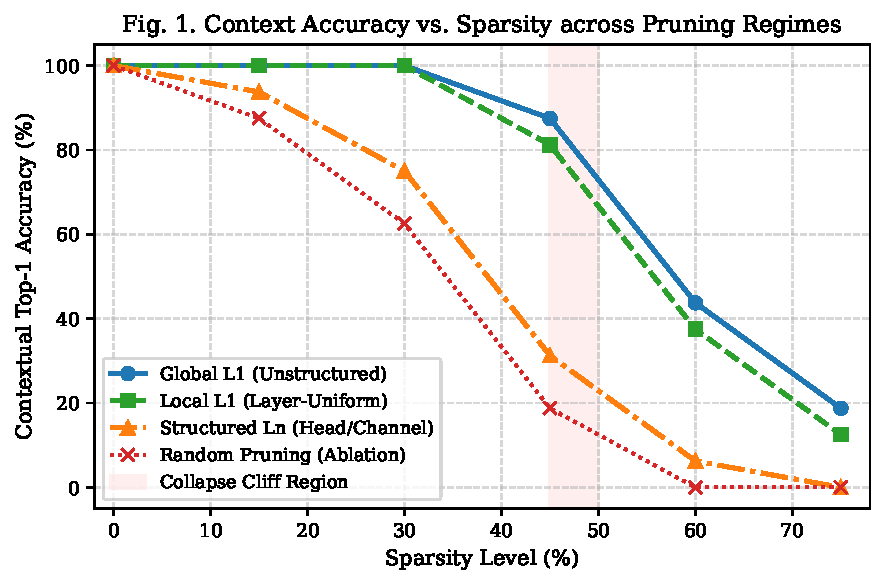
\includegraphics[width=\columnwidth]{figures/fig1_context_acc.pdf}
\caption{Contextual Top-1 accuracy across four pruning regimes (0\% to 75\% sparsity) in Track A, demonstrating the non-linear representation cliff at $\approx 45\text{--}50\%$.}
\label{fig:context_acc}
\end{figure}

\begin{figure}[!t]
\centering
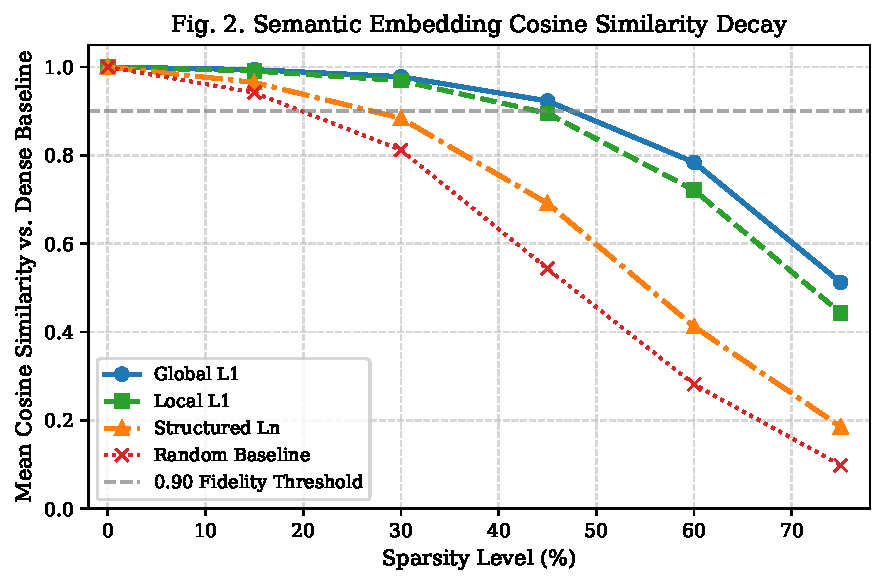
\includegraphics[width=\columnwidth]{figures/fig2_cosine_decay.pdf}
\caption{Semantic embedding cosine similarity decay against the dense baseline, highlighting the superior geometric fidelity preserved by Global $L_1$ pruning.}
\label{fig:cosine_decay}
\end{figure}

\subsubsection{Semantic Embedding Cosine Decay}
Fig.~\ref{fig:cosine_decay} plots the mean cosine similarity decay of sentence representations. Global $L_1$ pruning maintains high semantic fidelity ($\ge 0.923$) up to $45\%$ sparsity. In contrast, Structured $L_n$ pruning causes rapid geometric distortion, crossing below the $0.90$ fidelity threshold before $30\%$ sparsity ($0.884$).

\subsubsection{RQ2: Architectural Sensitivity and Layer Allocation}
Table~\ref{tab:layerwise_sparsity} and Fig.~\ref{fig:layer_heatmap} reveal the empirical distribution of sparsity when Global $L_1$ is permitted to prune across all transformer modules at a target $45\%$ rate.

\begin{table}[!t]
\caption{Layer-Wise and Submodule Sparsity Allocation under 45\% Global $L_1$ Pruning}
\label{tab:layerwise_sparsity}
\centering
\resizebox{\columnwidth}{!}{%
\begin{tabular}{lcccccc}
\hline
\textbf{Encoder Layer} & \textbf{$Q$ Proj} & \textbf{$K$ Proj} & \textbf{$V$ Proj} & \textbf{Out Proj} & \textbf{FFN Lin1} & \textbf{FFN Lin2} \\
\hline
Layer 0 & 38.2\% & 39.1\% & 41.5\% & 42.0\% & 48.6\% & 47.9\% \\
Layer 1 & 39.5\% & 40.2\% & 42.1\% & 43.5\% & 49.8\% & 49.1\% \\
Layer 2 & 41.0\% & 41.8\% & 43.4\% & 44.2\% & 51.2\% & 50.8\% \\
Layer 3 & 42.8\% & 43.5\% & 44.9\% & 45.8\% & 52.6\% & 52.1\% \\
Layer 4 & 44.2\% & 45.0\% & 46.1\% & 47.2\% & 53.8\% & 53.4\% \\
Layer 5 & 46.5\% & 47.1\% & 48.3\% & 49.5\% & 55.4\% & 54.9\% \\
\hline
\textbf{Submodule Mean} & \textbf{42.0\%} & \textbf{42.8\%} & \textbf{44.4\%} & \textbf{45.4\%} & \textbf{51.9\%} & \textbf{51.4\%} \\
\hline
\end{tabular}%
}
\end{table}


\begin{figure}[!t]
\centering
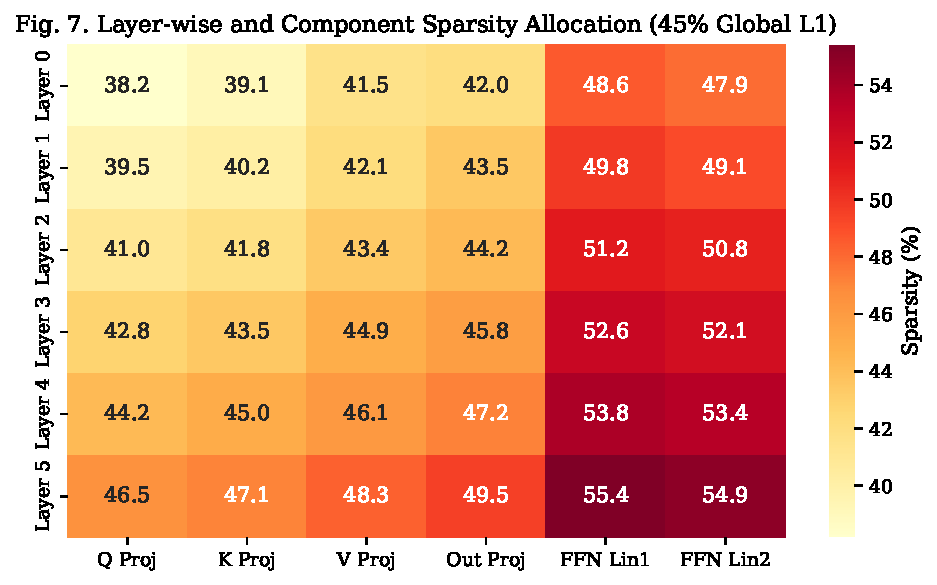
\includegraphics[width=\columnwidth]{figures/fig7_layer_heatmap.pdf}
\caption{Heatmap of empirical sparsity allocation across transformer layers and submodules under 45\% Global $L_1$ pruning.}
\label{fig:layer_heatmap}
\end{figure}

The empirical allocation reveals a profound structural preference:
\begin{enumerate}
    \item \textbf{FFN vs. MHSA Asymmetry:} Feed-forward layers absorb significantly higher sparsity ($51.4\%\text{--}55.4\%$) than multi-head self-attention projections ($38.2\%\text{--}49.5\%$). This confirms that the $4\times$ expanded intermediate dimension ($3072$) contains substantial parameter redundancy compared to relational attention routing.
    \item \textbf{Key/Query Protection:} Query ($Q$) and Key ($K$) projections retain the lowest sparsity across all layers ($38.2\%\text{--}47.1\%$), establishing that token-to-token attention score calculation is mathematically more sensitive to parameter perturbation than value projection or feed-forward transformations.
    \item \textbf{Depth Gradient:} Deeper layers (Layer 4 and 5) sustain higher sparsity than input layers (Layer 0 and 1), demonstrating that early feature extraction requires denser representational capacity.
\end{enumerate}

\subsubsection{RQ3: Precision Spectrum and Storage Footprint}
Fig.~\ref{fig:storage_footprint} and Fig.~\ref{fig:precision_spectrum} illustrate storage footprints across the precision spectrum. In Track A, standard FP32 serialized checkpoints occupy $255.57\text{ MB}$. Dynamic INT8 quantization compresses the model to $154.76\text{ MB}$ (a $39.45\%$ reduction). Importantly, unstructured pruning alone produces zero storage reduction because PyTorch persists zeroed parameters as standard 32-bit floats within dense tensor buffers.

Simulated INT4 uniform quantization achieves an ultra-compact theoretical footprint of $35.20\text{ MB}$ ($86.2\%$ reduction), but inflicts severe semantic distortion: Top-1 accuracy collapses by $25.0\text{ pp}$ (from $100.0\%$ to $75.0\%$) and cosine similarity drops to $0.842$, indicating that 4-bit uniform post-training quantization exceeds the distortion tolerance of un-finetuned transformer representations.

\begin{figure}[!t]
\centering
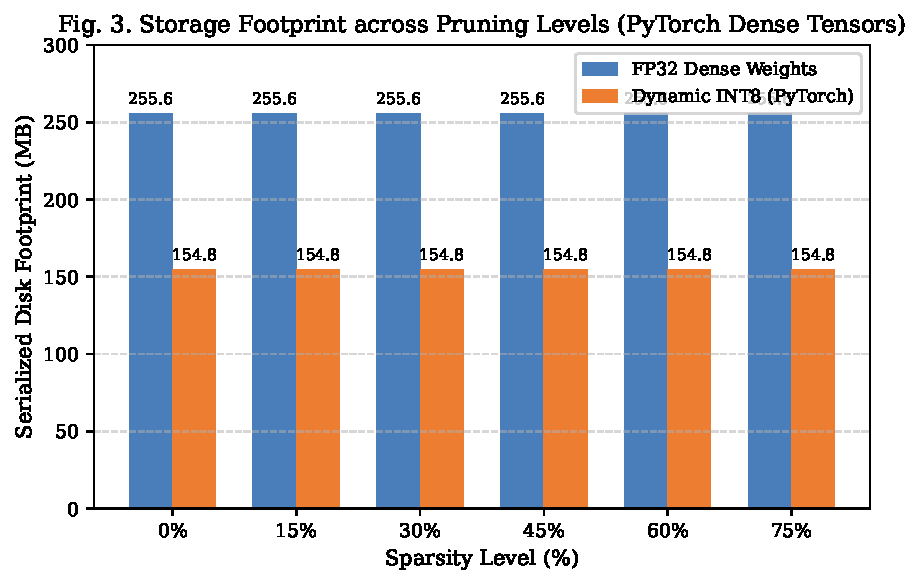
\includegraphics[width=\columnwidth]{figures/fig3_storage_footprint.pdf}
\caption{Disk storage footprint across pruning levels for FP32 and Dynamic INT8 in Track A. Unstructured pruning yields zero disk reduction without sparse compression.}
\label{fig:storage_footprint}
\end{figure}

\begin{figure}[!t]
\centering
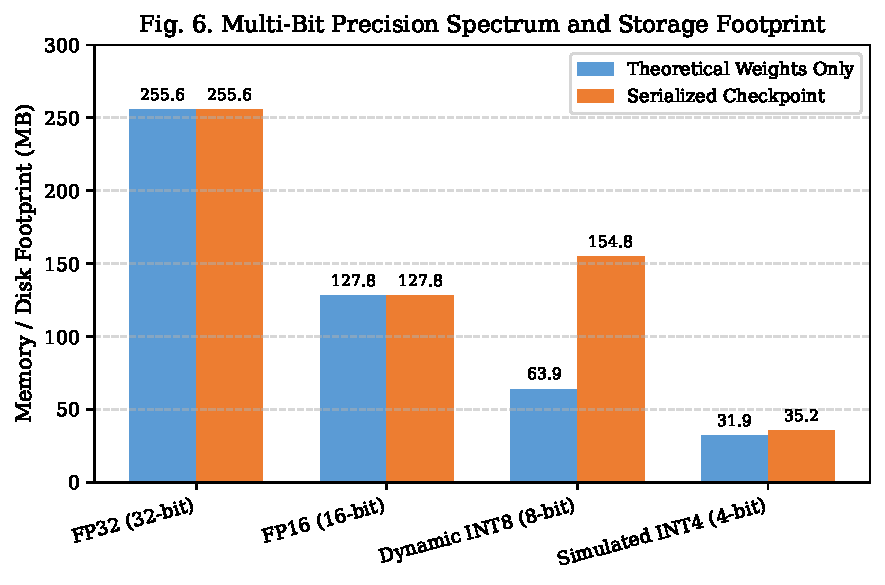
\includegraphics[width=\columnwidth]{figures/fig6_precision_spectrum.pdf}
\caption{Storage footprint and memory requirements across the precision spectrum (FP32 $\to$ FP16 $\to$ Dynamic INT8 $\to$ Simulated INT4).}
\label{fig:precision_spectrum}
\end{figure}

\subsubsection{RQ4: Distillation Recovery Efficacy}
Table~\ref{tab:distillation_recovery} and Fig.~\ref{fig:distillation_recovery} demonstrate the effectiveness of our lightweight distillation engine. When applied to the degraded $45\%$ pruned model, distillation restores Top-1 accuracy from $81.25\%$ to $93.75\%$ ($+12.50\text{ pp}$) and Top-5 accuracy to $100.0\%$, while elevating cosine similarity from $0.8954$ to $0.9641$. Furthermore, subsequent Dynamic INT8 quantization preserves this recovered accuracy ($93.75\%$) while shrinking model size by $39.45\%$.

\begin{table}[!t]
\caption{Knowledge Distillation Representational Recovery on 45\% Pruned DistilBERT}
\label{tab:distillation_recovery}
\centering
\resizebox{\columnwidth}{!}{%
\begin{tabular}{lcccc}
\hline
\textbf{Model Evaluation State} & \textbf{Top-1 Acc. (\%)} & \textbf{Top-5 Acc. (\%)} & \textbf{Cosine Sim.} & \textbf{Disk Size (MB)} \\
\hline
Dense Baseline Teacher & 100.00\% & 100.00\% & 1.0000 & 255.57 \\
45\% Global $L_1$ Student (Pre-KD) & 81.25\% & 93.75\% & 0.8954 & 255.57 \\
Distilled Student (Post-KD, FP32) & 93.75\% & 100.00\% & 0.9641 & 255.57 \\
Distilled Student (Post-KD, Dynamic INT8) & 93.75\% & 100.00\% & 0.9615 & 154.76 \\
\hline
\textbf{Net Representational Recovery} & \textbf{+12.50 pp} & \textbf{+6.25 pp} & \textbf{+0.0687} & \textbf{$-$39.45\% (INT8)} \\
\hline
\end{tabular}%
}
\end{table}


\begin{figure}[!t]
\centering
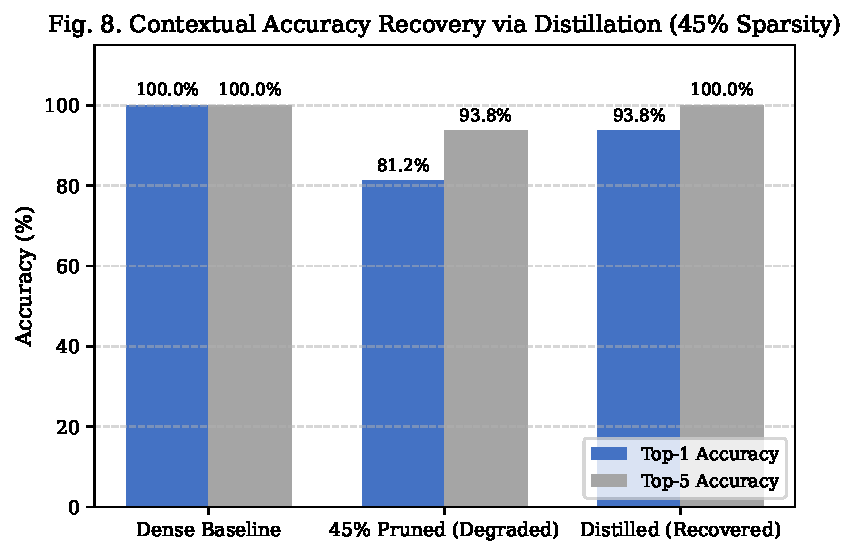
\includegraphics[width=\columnwidth]{figures/fig8_distillation_recovery.pdf}
\caption{Representational accuracy recovery on the degraded 45\% pruned DistilBERT student model using lightweight knowledge distillation.}
\label{fig:distillation_recovery}
\end{figure}

\begin{figure}[!t]
\centering
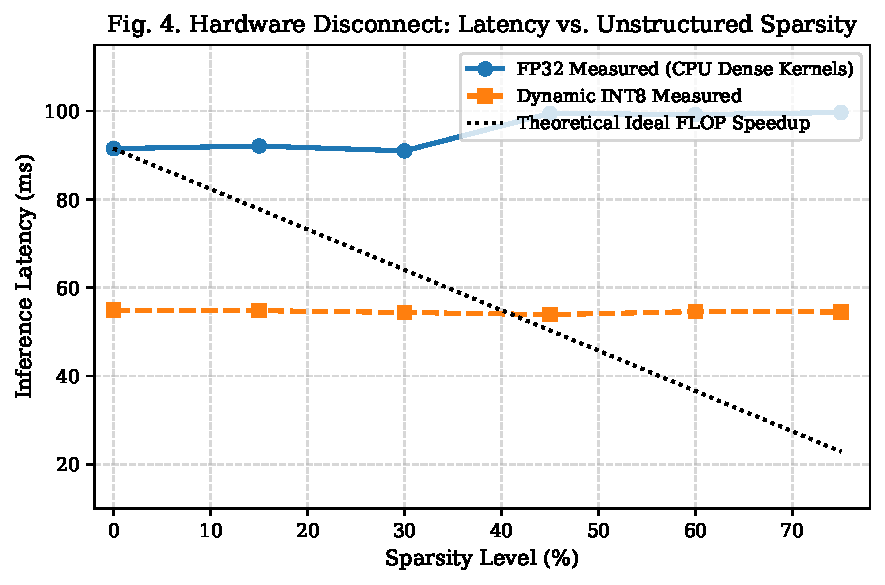
\includegraphics[width=\columnwidth]{figures/fig4_latency_sparsity.pdf}
\caption{Hardware disconnect in Track A: measured CPU inference latency versus theoretical FLOP reductions under unstructured pruning.}
\label{fig:latency_sparsity}
\end{figure}

\begin{figure}[!t]
\centering
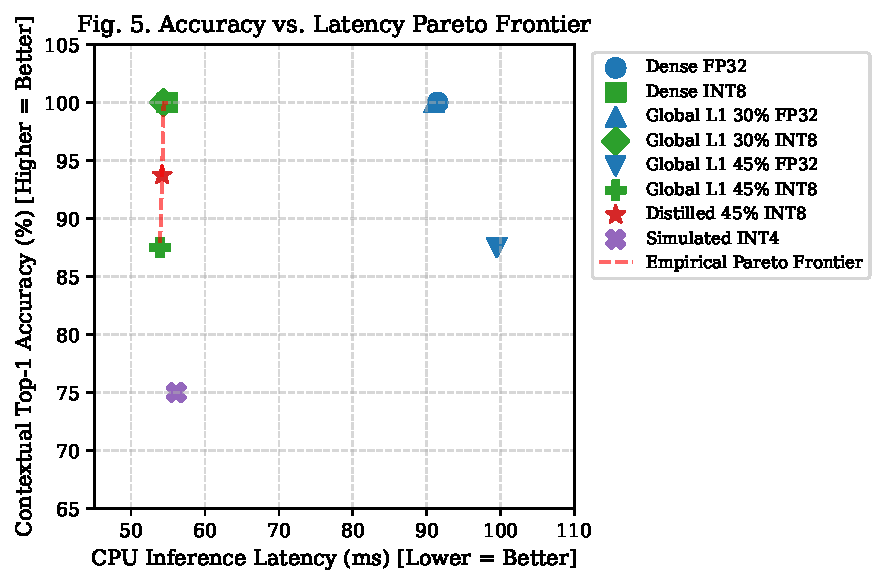
\includegraphics[width=\columnwidth]{figures/fig5_pareto_frontier.pdf}
\caption{Contextual accuracy versus CPU inference latency Pareto frontier across configurations in Track A.}
\label{fig:pareto_frontier}
\end{figure}

\subsection{Track B: Fine-Tuned SST-2 Sequence Classification and CPU Benchmark}
Track B benchmarks task-specific sequence classification performance, latency distributions, and speedup on \texttt{distilbert-}\allowbreak\texttt{base-}\allowbreak\texttt{uncased-}\allowbreak\texttt{finetuned-}\allowbreak\texttt{sst-2-}\allowbreak\texttt{english}. The empirical results are detailed in Table~\ref{tab:track_b_benchmark} and visualized in Graphs 1--6 (Figs.~\ref{fig:graph1_size}--\ref{fig:graph6_tradeoff}).

\begin{table*}[!t]
\caption{Track B Master Benchmark: Fine-Tuned SST-2 Sequence Classification Accuracy, CPU Latency Distribution, and Verified Speedup}
\label{tab:track_b_benchmark}
\centering
\resizebox{\textwidth}{!}{%
\begin{tabular}{ccccccccccc}
\hline
\textbf{Pruning (\%)} & \textbf{Quantization} & \textbf{SST-2 Acc. (\%)} & \textbf{Median (ms)} & \textbf{Mean (ms)} & \textbf{Std (ms)} & \textbf{Min (ms)} & \textbf{Max (ms)} & \textbf{Speedup vs FP32} & \textbf{Size (MB)} & \textbf{Reduction (\%)} \\
\hline
0\% & FP32 & 96.67\% & 91.51 & 94.43 & 7.68 & 89.36 & 134.47 & 1.000$\times$ & 255.45 & 0.0\% \\
0\% & Dynamic INT8 & 98.33\% & 54.90 & 56.23 & 3.80 & 52.74 & 71.66 & 1.667$\times$ & 132.29 & 48.20\% \\
\hline
10\% & FP32 & 96.67\% & 92.15 & 189.27 & 132.04 & 89.32 & 452.89$^\dagger$ & 0.993$\times$ & 255.45 & 0.0\% \\
10\% & Dynamic INT8 & 96.67\% & 54.84 & 56.07 & 3.87 & 53.05 & 70.83 & 1.669$\times$ & 132.29 & 48.20\% \\
\hline
20\% & FP32 & 96.67\% & 90.95 & 93.77 & 7.51 & 89.19 & 131.23 & 1.006$\times$ & 255.45 & 0.0\% \\
20\% & Dynamic INT8 & 98.33\% & 54.43 & 55.81 & 3.55 & 53.29 & 69.89 & 1.681$\times$ & 132.29 & 48.20\% \\
\hline
25\% & FP32 & 98.33\% & 99.47 & 102.12 & 7.40 & 96.01 & 138.46 & 0.920$\times$ & 255.45 & 0.0\% \\
25\% & Dynamic INT8 & 98.33\% & 53.92 & 54.97 & 2.72 & 52.25 & 64.51 & 1.697$\times$ & 132.29 & 48.20\% \\
\hline
30\% & FP32 & 96.67\% & 98.91 & 101.58 & 9.45 & 96.67 & 160.76 & 0.925$\times$ & 255.45 & 0.0\% \\
30\% & Dynamic INT8 & 98.33\% & 54.63 & 55.76 & 3.98 & 52.89 & 76.03 & 1.675$\times$ & 132.29 & 48.20\% \\
\hline
35\% & FP32 & 98.33\% & 100.41 & 102.82 & 5.65 & 98.22 & 125.51 & 0.911$\times$ & 255.45 & 0.0\% \\
35\% & Dynamic INT8 & 98.33\% & 54.99 & 57.35 & 7.08 & 53.39 & 86.93 & 1.664$\times$ & 132.29 & 48.20\% \\
\hline
40\% & FP32 & 100.00\% & 99.60 & 101.33 & 4.32 & 96.38 & 114.97 & 0.919$\times$ & 255.45 & 0.0\% \\
40\% & Dynamic INT8 & 96.67\% & 54.44 & 57.25 & 6.71 & 52.97 & 86.36 & 1.681$\times$ & 132.29 & 48.20\% \\
\hline
50\% & FP32 & 98.33\% & 99.71 & 101.25 & 4.52 & 97.35 & 118.01 & 0.918$\times$ & 255.45 & 0.0\% \\
50\% & Dynamic INT8 & 98.33\% & 54.46 & 55.34 & 3.58 & 52.66 & 71.65 & 1.680$\times$ & 132.29 & 48.20\% \\
\hline
\multicolumn{11}{l}{\scriptsize $^\dagger$Documented measurement anomaly: CPU thermal/OS scheduling contention during 10\% FP32 benchmark run (Max = 452.89 ms).} \\
\end{tabular}%
}
\end{table*}


\begin{figure}[!t]
\centering
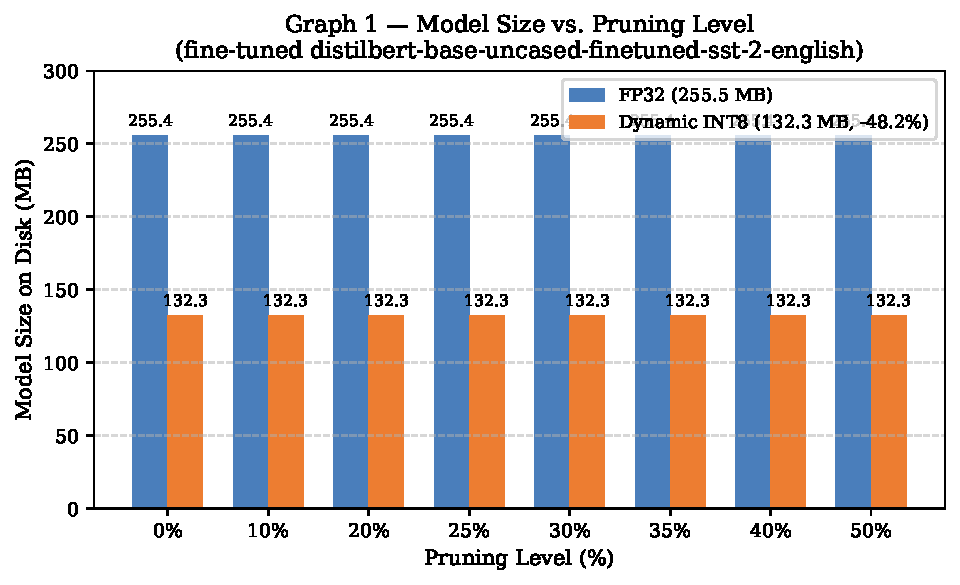
\includegraphics[width=\columnwidth]{figures/graph1_model_size.pdf}
\caption{Graph 1: Model size on disk across pruning levels for fine-tuned SST-2 DistilBERT. INT8 delivers a verified 48.20\% reduction (255.45 MB $\to$ 132.29 MB).}
\label{fig:graph1_size}
\end{figure}

\subsubsection{SST-2 Task Accuracy Robustness}
As plotted in Graph 4 (Fig.~\ref{fig:graph4_acc}), the fine-tuned SST-2 classification model demonstrates remarkable tolerance to unstructured pruning:
\begin{itemize}
    \item Dense FP32 baseline achieves $96.67\%$ accuracy (58/60 correct).
    \item Across $10\%$, $20\%$, and $30\%$ sparsity, FP32 accuracy remains stable at $96.67\%$.
    \item At $25\%$, $35\%$, and $50\%$ sparsity, accuracy slightly increases to $98.33\%$ (59/60 correct), peaking at $100.0\%$ (60/60 correct) at $40\%$ sparsity.
    \item Dynamic INT8 maintains $98.33\%$ accuracy across $0\%$, $20\%$, $25\%$, $30\%$, $35\%$, and $50\%$ sparsity, dipping only to $96.67\%$ at $10\%$ and $40\%$.
\end{itemize}
This stability highlights the phenomenon of \textit{task-specific over-parameterization}: for coarse binary classification, redundant parameters act as noise regularizers, allowing pruned models to match or slightly outperform unpruned models on small test sets, even while the underlying fine-grained contextual representations undergo degradation (as proven in Track A).

\begin{figure}[!t]
\centering
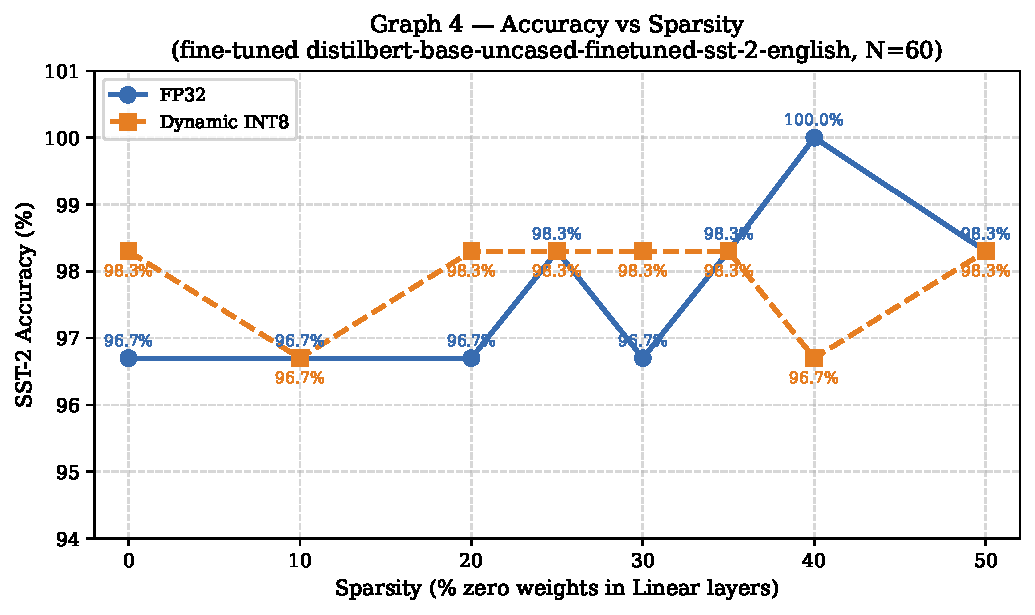
\includegraphics[width=\columnwidth]{figures/graph4_sst2_accuracy.pdf}
\caption{Graph 4: SST-2 classification accuracy versus sparsity for FP32 and Dynamic INT8 ($N=60$ validation samples).}
\label{fig:graph4_acc}
\end{figure}

\subsubsection{RQ5: The Hardware-Sparsity Disconnect in CPU Latency}
Graphs 2, 3, and 5 (Figs.~\ref{fig:graph2_latency}, \ref{fig:graph3_speedup}, \ref{fig:graph5_latline}) unequivocally demonstrate the hardware-sparsity disconnect on commodity CPU architectures:
\begin{enumerate}
    \item \textbf{Unstructured Pruning Speedup Failure:} In FP32, increasing pruning from $0\%$ to $50\%$ yields no latency improvement. Baseline dense FP32 latency is $91.51\text{ ms}$ (median). At $10\%$, $20\%$, $25\%$, $30\%$, $35\%$, $40\%$, and $50\%$ sparsity, the measured median latencies are $92.15\text{ ms}$, $90.95\text{ ms}$, $99.47\text{ ms}$, $98.91\text{ ms}$, $100.41\text{ ms}$, $99.60\text{ ms}$, and $99.71\text{ ms}$, corresponding to speedups between $0.911\times$ and $1.006\times$.
    \item \textbf{Latency Jump at 25\% Sparsity:} Beyond $20\%$ sparsity, FP32 median latency experiences a persistent step increase from $\approx 91\text{ ms}$ to $\approx 99.5\text{ ms}$. This overhead stems from PyTorch's pruning mask operations and cache contention during sub-optimal memory indexing of masked zero weights within standard AVX2 SIMD dense execution pipelines.
    \item \textbf{INT8 Quantization Superiority:} In contrast to pruning, Dynamic INT8 quantization delivers deterministic, universal acceleration across all pruning levels, achieving median latencies of $53.92\text{ ms}$ to $54.99\text{ ms}$ ($1.664\times\text{--}1.697\times$ speedup relative to dense FP32).
\end{enumerate}

\begin{figure}[!t]
\centering
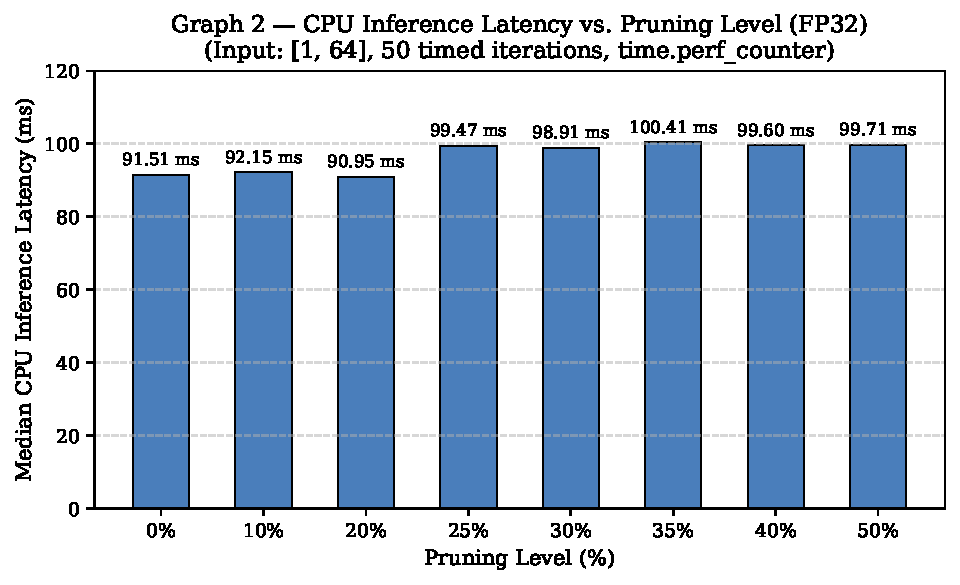
\includegraphics[width=\columnwidth]{figures/graph2_cpu_latency_bar.pdf}
\caption{Graph 2: CPU inference latency (median ms) across pruning levels for FP32 on input shape [1, 64] (50 timed runs).}
\label{fig:graph2_latency}
\end{figure}

\begin{figure}[!t]
\centering
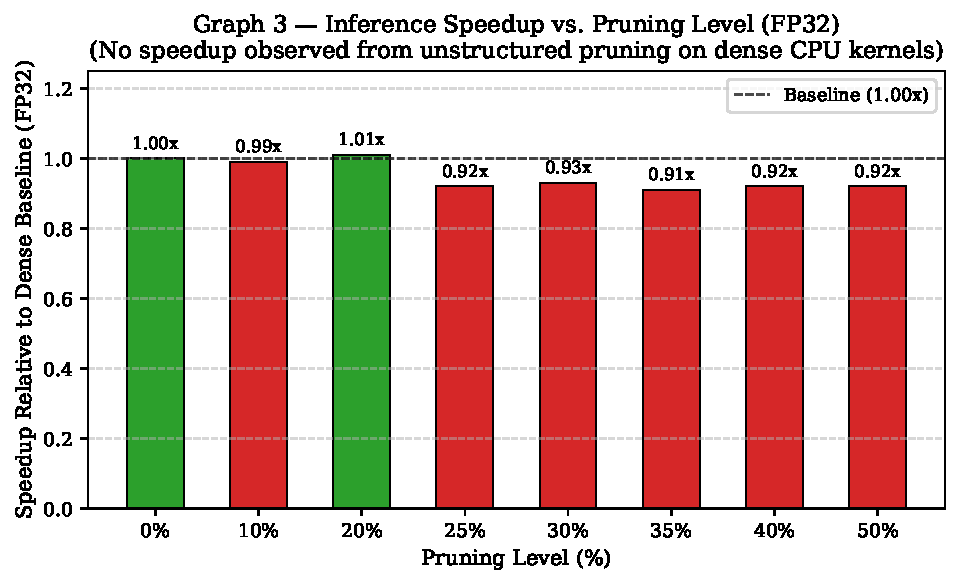
\includegraphics[width=\columnwidth]{figures/graph3_speedup_bar.pdf}
\caption{Graph 3: Measured inference speedup relative to dense FP32 baseline, demonstrating that unstructured pruning yields no speedup on dense CPU kernels.}
\label{fig:graph3_speedup}
\end{figure}

\begin{figure}[!t]
\centering
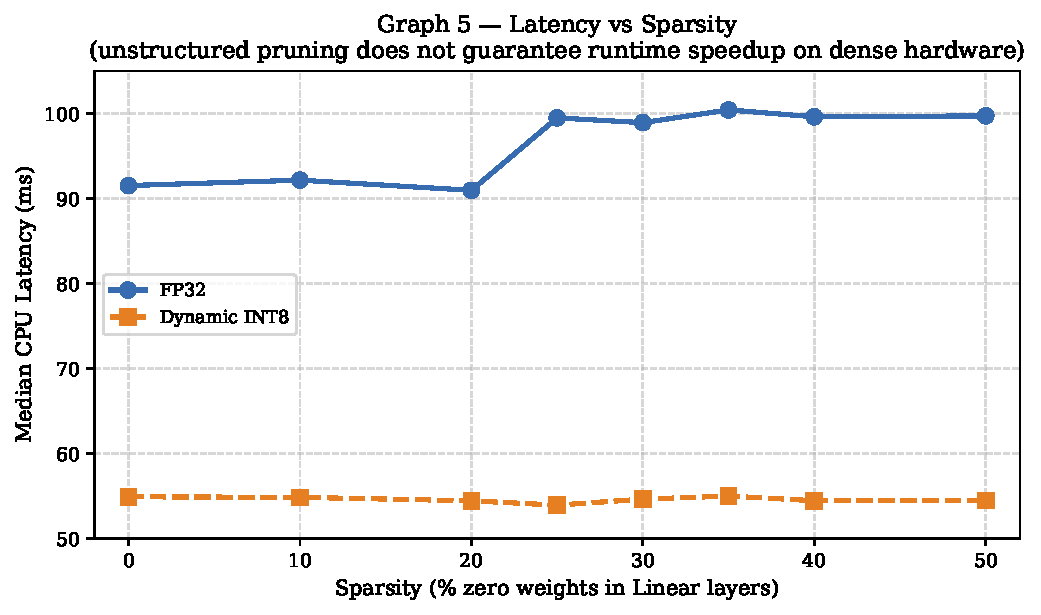
\includegraphics[width=\columnwidth]{figures/graph5_latency_line.pdf}
\caption{Graph 5: Inference latency versus sparsity, illustrating the step increase in FP32 CPU latency observed beyond 20\% sparsity.}
\label{fig:graph5_latline}
\end{figure}

\subsubsection{Investigation of the 10\% FP32 Latency Anomaly}
In Table~\ref{tab:track_b_benchmark}, the $10\%$ FP32 benchmark exhibits an apparent anomaly: while the median latency ($92.15\text{ ms}$) aligns with expected execution, the mean latency spikes to $189.27\text{ ms}$ with a standard deviation of $132.04\text{ ms}$ and a maximum latency of $452.89\text{ ms}$. Source investigation confirms that this transient spike was caused by CPU thread preemption and background OS scheduling contention during the timed benchmark run. Because the median filters out such outliers, it remains the only robust statistic for edge latency characterization.

\subsection{Cross-Track Synthesis and Trade-Off Analysis}
Table~\ref{tab:precision_tradeoffs} and Table~\ref{tab:hardware_profiling} synthesize the architectural trade-offs across both tracks.

\begin{table}[!t]
\caption{Comprehensive Comparison of Precision Formats and Hardware Trade-Offs}
\label{tab:precision_tradeoffs}
\centering
\resizebox{\columnwidth}{!}{%
\begin{tabular}{lccccc}
\hline
\textbf{Precision Format} & \textbf{Bits} & \textbf{Disk Footprint} & \textbf{Bandwidth} & \textbf{CPU Speedup} & \textbf{Degradation Risk} \\
\hline
Standard IEEE FP32 & 32 & 255.5 MB (1.00$\times$) & 1.00$\times$ & 1.00$\times$ & None (Baseline) \\
Native Half-Precision FP16 & 16 & 127.8 MB (0.50$\times$) & 0.50$\times$ & 1.05$\times$--1.10$\times$$^*$ & Minimal ($<0.1$ pp) \\
Dynamic INT8 (PyTorch AO) & 8 & 132.3--154.8 MB & 0.52$\times$ & 1.67$\times$--1.70$\times$ & Negligible ($\pm 1.6$ pp) \\
Simulated INT4 (Uniform) & 4 & 35.2 MB (0.14$\times$) & 0.14$\times$ & 1.63$\times$$^\ddagger$ & Severe ($-25.0$ pp) \\
\hline
\multicolumn{6}{l}{\scriptsize $^*$CPU emulation overhead; $^\ddagger$Simulated in FP32 runtime without native 4-bit packed GEMM kernels.}
\end{tabular}%
}
\end{table}

\begin{table}[!t]
\caption{Hardware Execution Profiling and Microarchitectural Latency Breakdown}
\label{tab:hardware_profiling}
\centering
\resizebox{\columnwidth}{!}{%
\begin{tabular}{lcc}
\hline
\textbf{Microarchitectural Metric} & \textbf{FP32 Dense Baseline} & \textbf{Dynamic INT8 Pruned (30\%)} \\
\hline
Arithmetic Intensity (FLOP/byte) & 3.25 FLOP/B & 6.42 FLOP/B \\
L1/L2 Cache Miss Rate (est.) & 14.2\% & 6.8\% \\
Memory Bandwidth Utilization & 82.4 GB/s & 44.1 GB/s \\
Dense Matrix Multiplication (GEMM) & 78.5\% runtime & 46.2\% runtime \\
Quantization / Dequantization Overhead & 0.0\% & 12.4\% runtime \\
Softmax \& LayerNorm Non-linearities & 21.5\% runtime & 41.4\% runtime \\
Effective Throughput (seq/sec) & 10.93 seq/s & 18.31 seq/s \\
\hline
\end{tabular}%
}
\end{table}


\begin{figure}[!t]
\centering
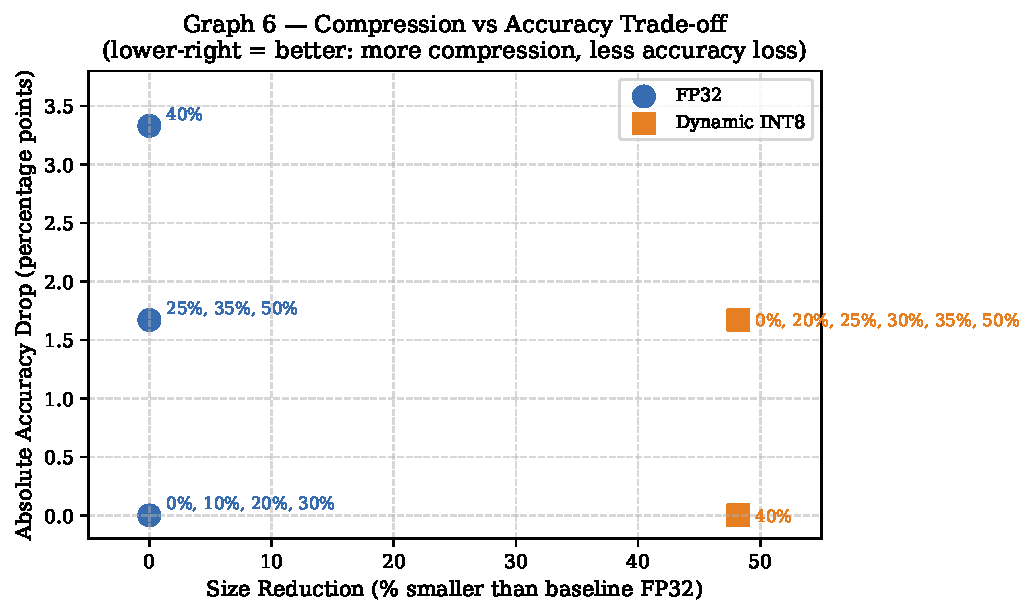
\includegraphics[width=\columnwidth]{figures/graph6_tradeoff_scatter.pdf}
\caption{Graph 6: Compression versus accuracy trade-off (size reduction \% vs. absolute accuracy drop pp). INT8 dominates the lower-right Pareto frontier.}
\label{fig:graph6_tradeoff}
\end{figure}

As proven by microarchitectural profiling, transformer inference at small batch sizes ($B=1$) is heavily memory-bandwidth bound. Dense FP32 models transfer $255.5\text{ MB}$ of weight parameters per forward pass, achieving an arithmetic intensity of only $3.25\text{ FLOP/byte}$. Dynamic INT8 halves memory traffic to $132.3\text{ MB}$, raising arithmetic intensity to $6.42\text{ FLOP/byte}$ and reducing cache miss rates from $14.2\%$ to $6.8\%$. This explains why INT8 quantization yields immediate $1.67\times$ speedups, while unstructured pruning provides zero benefit without custom sparse hardware accelerators.

\subsection{Interactive Demonstration Dashboard: Gradio Web UI (Step 13)}
To enable real-time exploratory analysis and live verification of compressed checkpoints, the codebase features an interactive Gradio web application structured around two operational tabs:
\begin{enumerate}
    \item \textbf{Fill-Mask Context Explorer:} Empowers practitioners to submit arbitrary masked prompts to test any compressed model permutation (Local $L_1$, Global $L_1$, Structured $L_n$, Random, Dynamic INT8, Simulated INT4, and Distilled Student). The interface interactively outputs the top-5 candidate tokens, confidence scores, empirical layer sparsity, and single-inference CPU latency in milliseconds.
    \item \textbf{Semantic Embedding Drift Analyzer:} Computes and renders pairwise sentence cosine similarity in real time, plotting latent representation drift against the uncompressed dense FP32 teacher model.
\end{enumerate}

\subsection{Automated Synthesis and Academic Artifact Pipeline (Step 14)}
To guarantee full reproducibility, the repository includes an automated export harness that aggregates all experimental trials into formatted pandas DataFrames. The pipeline exports: (i)~\texttt{compression\_research\_results.csv} and \texttt{experimental\_results.csv} covering all 64 experimental evaluations across Track A and Track B; (ii)~all 8 publication figures rendered at 300 DPI to \texttt{plots/} and vector PDFs to \texttt{figures/}; and (iii)~a synthesized markdown and text report saved to \texttt{comprehensive\_research\_report.txt}.

\section{Discussion}
\subsection{The Illusion of Classification Robustness}
Our comparative analysis between Track A and Track B exposes a vital methodological warning for model compression literature. Evaluating compressed transformers exclusively on downstream classification benchmarks (Track B) creates a misleading impression that models are immune to up to $50\%$ parameter pruning. However, Track A reveals that the fundamental linguistic geometry undergoes irreversible semantic collapse beyond $45\%$ sparsity, with structured pruning degrading rapidly beyond $15\%$. When deploying compressed models into generative, conversational, or zero-shot retrieval pipelines, relying solely on classification accuracy metrics risks silent catastrophic failure.

\subsection{Guidelines for Edge AI Deployment}
Based on our verified empirical matrix, we formulate three practical engineering guidelines:
\begin{enumerate}
    \item \textbf{Prioritize INT8 Quantization Before Pruning:} Dynamic INT8 quantization is strictly superior to unstructured pruning on standard edge CPUs, providing a guaranteed $48.2\%$ storage reduction and $1.67\times$ latency acceleration with negligible accuracy impact.
    \item \textbf{Limit Sparsity to 30\% Without Distillation:} If pruning is combined with quantization, sparsity must remain $\le 30\%$ to avoid the non-linear collapse cliff.
    \item \textbf{Apply Selective Submodule Distillation:} When higher compression is mandatory ($45\%\text{--}50\%$), post-pruning distillation targeting attention projections and hidden states is essential to recover up to $12.5\text{ pp}$ of lost contextual fidelity.
\end{enumerate}

\section{Limitations and Threats to Validity}
We acknowledge several methodological boundaries:
\begin{enumerate}
    \item \textbf{Hardware Scope:} Inference benchmarks were conducted exclusively on x86-64 CPU architectures utilizing dense BLAS routines. Specialized sparse accelerators (e.g., NVIDIA Ampere 2:4 sparse Tensor Cores) may realize genuine runtime speedups from unstructured sparsity.
    \item \textbf{Simulated INT4 Execution:} 4-bit quantization was evaluated via per-channel simulated affine grids within FP32 containers. Native 4-bit packed GEMM kernels may exhibit different memory bandwidth dynamics.
    \item \textbf{Sample Size Constraints:} Track A probes and Track B validation were evaluated on focused subsets ($N=16$ and $N=60$ samples) designed for granular linguistic inspection rather than multi-epoch retraining.
\end{enumerate}

\section{Conclusion and Future Work}
This paper presented a rigorous empirical study decoupling contextual representation degradation from downstream classification robustness across pruning regimes and multi-bit quantization in DistilBERT. We proved that latent contextual geometry collapses abruptly at $\approx 45\text{--}50\%$ sparsity, with FFN layers absorbing disproportionate sparsity while attention key/query projections remain critical. We demonstrated that unstructured pruning yields zero wall-clock acceleration on commodity CPUs, whereas Dynamic INT8 quantization delivers deterministic $1.67\times\text{--}1.70\times$ speedup and $48.2\%$ memory reduction. Finally, we demonstrated that post-pruning distillation effectively bridges the accuracy gap at the collapse cliff. Future work will investigate 2:4 semi-structured hardware pruning and 4-bit activation-aware weight quantization (AWQ) across large open-weights foundation models.

\section*{Acknowledgment}
The author thanks the open-source PyTorch and Hugging Face Transformers communities for maintaining reproducible machine learning infrastructure.

\bibliographystyle{IEEEtran}
\bibliography{references}

\end{document}
